\chapter{Temporal Planning}
\label{sec:temporal_planning}


\section{Task List}

This section lists all the tasks to be performed. 

\begin{enumerate}
\item Project Management
\begin{enumerate}
\item Project's Scope - 9h
\item Temporal Planning - 6h
\item Budget and sustainability - 3h
\item First Presentation - 6h
\item Context and Bibliography - 15h
\item Degree's specialization specification - 10h
\item Final document and presentation - 20h
\end{enumerate}
\item Software design description - 40h
\item Analysis tools' research - 40h
\item Common set up for all SCRUM cycles - 40h
\item SCRUM iterations - 960h control cycles
\begin{enumerate}
\item Initial analysis and optimization decision
\item Optimization development
\item Implementation measurements
\end{enumerate}
\item Global performance analysis - 40h

\item Project Writing and Defence Preparation - 80h
\end{enumerate}

\section{Tasks Description}


\subsection{Project Management}

This task is the responsible for the whole project planning and specification and covers all the deliverables of the GEP course. 

\subsubsection{Resources list}

\begin{description}
\item [TexStudio,] \hfill \\ desktop application used for report writing
\item [GanttProject,] \hfill \\ desktop application for Gantt chart creation
\item [UPC Atenea,] \hfill \\ online platform for deliverables submission
\end{description}

\subsection{Software design description}

The project aims to optimize an already existing project. This means that the first thing to do before starting to work is to explore, execute and, in general, familiarize myself with the original code. This will lead to the design description of pyProCT software. 

\subsubsection{Resources list}
\label{subsec:familiarresources}

\begin{description}
\item [Git and Github,] \hfill \\ to use the code we need a Github account to fork the original project repository. Once forked we need a git-able OS, in this case Linux Mint 17, to clone it. 
\item [MareNostrum III account,] \hfill \\ for executing the code on the supercomputer and correctly assess it's performance as well as execution limitations for instrumentation purposes.
\item [SSH-able OS] \hfill \\ to establish secure shell connections to the MareNostrum III computer for the program execution.
\item [Paraver and other analysis tools,] \hfill \\ to ease the understanding process with execution diagrams. Also, on this first stage, I will start looking for the best available tools for the posterior analysis stage.

\end{description}

\subsection{Analysis tools' research}

Once the whole program execution and mechanics, the next step is to decide which analysis tools are going to be used. Paraver is going to be amongst them. This task needs to be done after getting familiar with the code because otherwise we could end up trying to use tools which are not compatible with the python version and packages used and the remote execution pipeline. 

It is important to note that this is mainly a research stage. This means that no consistent code modifications are going to be performed, just the necessary ones to ensure that the tools work well with the code.

As a big part of the project is going to be analysis, we set up first this research stage and an implementation/instrumentation one in order to correctly address the importance of this matter.

\subsubsection{Resources list}
See \hypertarget{subsec:familiarresources}{Code Familiarization resources list~\ref{subsec:familiarresources}}.

\subsection{Common set up for all SCRUM cycles}
\label{subsec:setup}

Once I am familiar with the code and the analysis tools have been chosen, the next step will be to instrument the code for it's preliminary analysis. The instrumentation should be deep enough to test all the possible implementations to be done, regardless they are performed on the matrix distances calculation, task level or scheduler level. 

On this stage we will also do a preliminar work aimed to automate and speed up as much as possible the code analysis and execution. On one hand, this will speed up the SCRUM iterations by automating the analysis and execution with tools like bash scripts, allowing us to focus on the actual development and analysis and avoid wasting time on repetitive task as graphs' generation or the remote execution. On the other hand, it will also help to avoid human errors on the execution parameters, analysis settings and environment configuration.

\subsubsection{Resources list}

The resources required for this stage are linked to the analysis tools decisions so they can not be listed until the first stage is finished.

However common resources for automation are required (i.e. bash scripts). The Linux Mint environment used provides this basic functionalities.

\subsection{SCRUM iterations}

As explained on the Scope of the Project document, the work flow will follow the analysis-implementation-analysis structure. Each cycle is going to have, at least, one control meeting for each three weeks of work. This way we will keep track of the optimization development and solve possible problems.

The first and major implementation is going to be the COMPSs refactoring. Being the most important optimization, all iterations are going to be focused on it till it's completely ended (including analysis). If there is time for other optimizations its schedules and constraints are going to be decided at the start of each cycle.

The work to be done on each phase of the iteration has already been specified on the Project's Scope document and requires no further description.


\subsubsection{Resources list}

The common requirements for each cycle are all the ones mentioned on the previous sections. Some optimizations may require new tools and resources so at the start of each iteration, on the preliminary analysis, a resource analysis and specification is going to be performed.

\subsection{Global performance analysis}

After finishing all the implementations decided, a global analysis is going to be performed. The aim of it will be to show not the changes introduced by each optimization but how these all behave and interact between them. Also the global speed up obtained, the final execution pipeline and conclusion fall into this section.

\subsubsection{Resources list}

This section requires no more resources than the needed to correctly reach this stage of the project. 


\section{Gantt and PERT charts}
\label{sec:gantt_pert}

This is the resulting Gantt and PERT charts for the described tasks.
\\
\\

\begin{figure}[h]
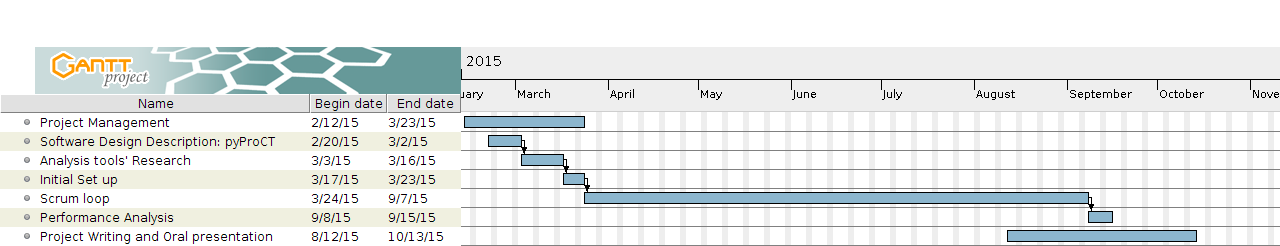
\includegraphics[width=\textwidth]{img/gantt.png}
\caption{Gantt Chart}
\end{figure}
\begin{figure}[h]
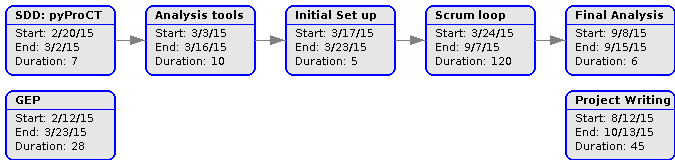
\includegraphics[width=\textwidth]{img/pert.png}
\caption{PERT Chart}
\end{figure}

\FloatBarrier
